\documentclass[main.tex]{subfiles}

\begin{document}

\section{Simulations}\label{sec:simulations}

In this chapter, we will test the previously described MPC in a virtual enviroment. Throughout the simulations, the whole complexity of the humanoid will be condensed in a single point, representing its CoM.\\
The objective of this set of tests is to prove that, using the inputs provided by the MPC proposed by Peng et al. in \cite{peng_main_paper} and developed by us, a robot is able to reach a user-defined goal, while avoiding collisions with all the obstacles in the environment.\\
The hyper-parameters used in the following simulations are summarized in Table \ref{table:sim_params}.

\begin{table}[h]
        \begin{tabular}{ |p{3cm}||p{3cm}|p{3cm}|p{3cm}|  }
             \hline
             \multicolumn{2}{|c|}{Simulation Parameters} \\
             \hline
             Parameter& Value\\
             \hline
             $\alpha$   & 1.44 \\
             %% TODO: add other parameters
             \hline
        \end{tabular}
    \centering
    \caption{The MPC and LIP parameters used for all the simulations in this chapter. \todo[inline]{add other parameters}}
    \label{table:sim_params}
\end{table}

\subsection{Simple Environment}
The first simulation takes place in a basic environment: the humanoid is positioned at $(0,\,0)$ with orientation $\theta = 0$, and the goal position is $(5,\,5)$. In between, we placed 5 obstacles with a randomly-generated convex shape. The results are shown in \todo[inline]{ADD IMAGE}. %TODO:

% EXAMPLE GRID
\begin{figure}[h]
    \centering
    % First row
    \begin{subfigure}{0.20\textwidth}
        \centering
        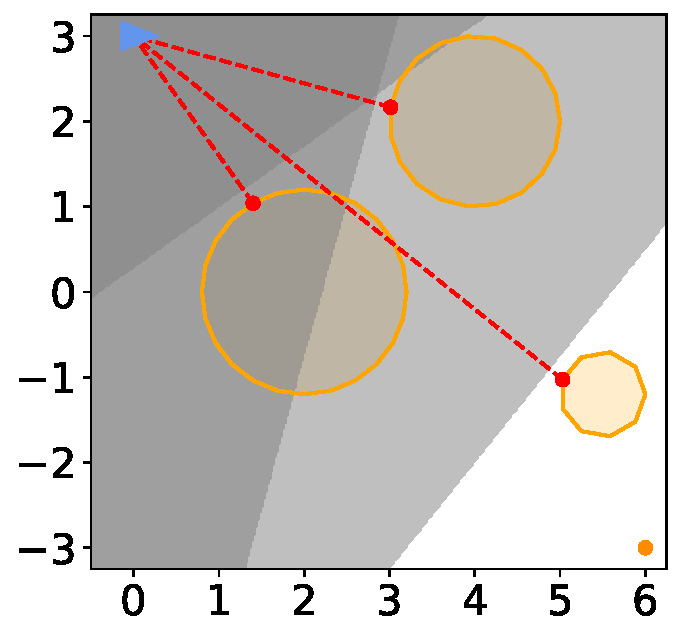
\includegraphics[width=\textwidth]{figures/Simulations/sim1/frame_0.pdf}
    \end{subfigure}%
    \hfill
    \begin{subfigure}{0.20\textwidth}
        \centering
        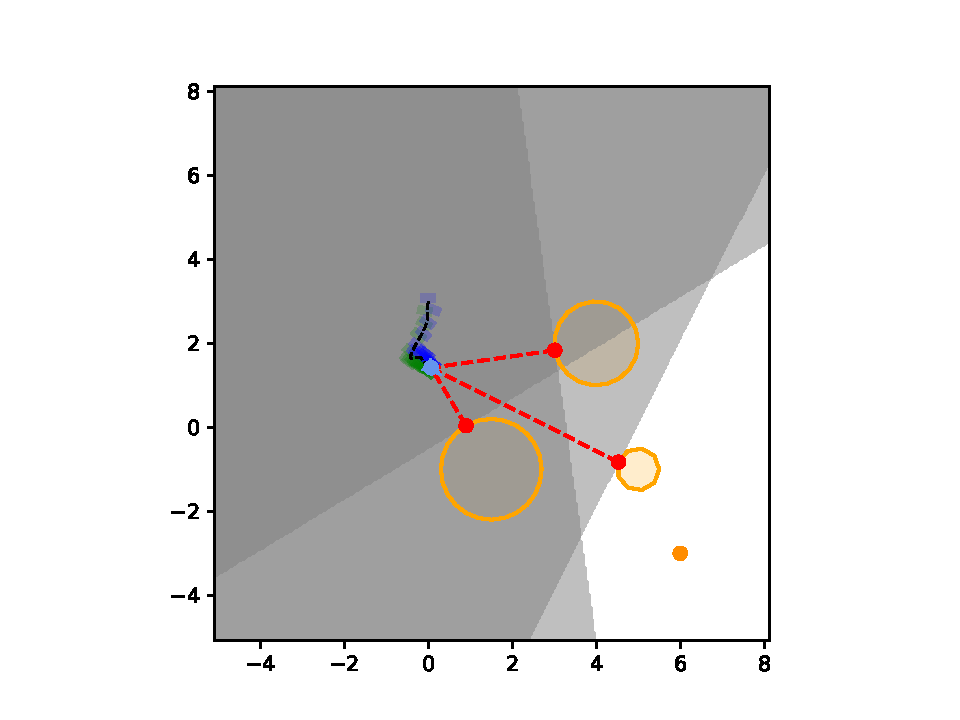
\includegraphics[width=\textwidth]{figures/Simulations/sim1/frame_1.pdf}
    \end{subfigure}%
    \hfill
    \begin{subfigure}{0.20\textwidth}
        \centering
        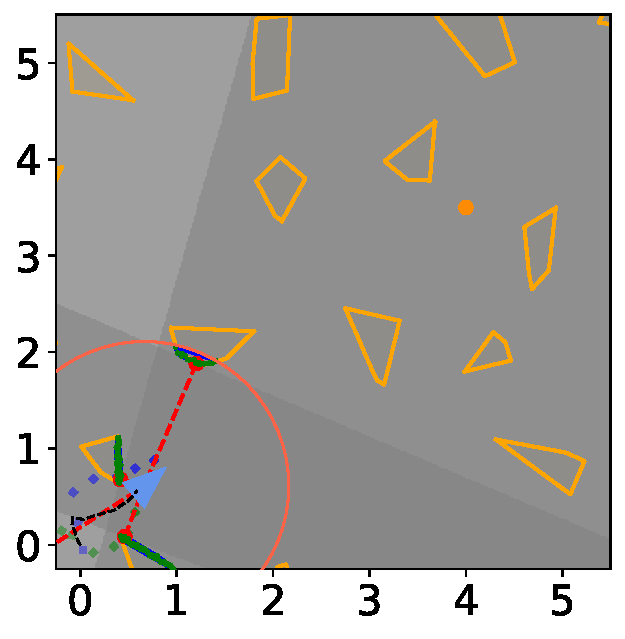
\includegraphics[width=\textwidth]{figures/Simulations/sim1/frame_2.pdf}
    \end{subfigure}%
    \hfill
    \begin{subfigure}{0.20\textwidth}
        \centering
        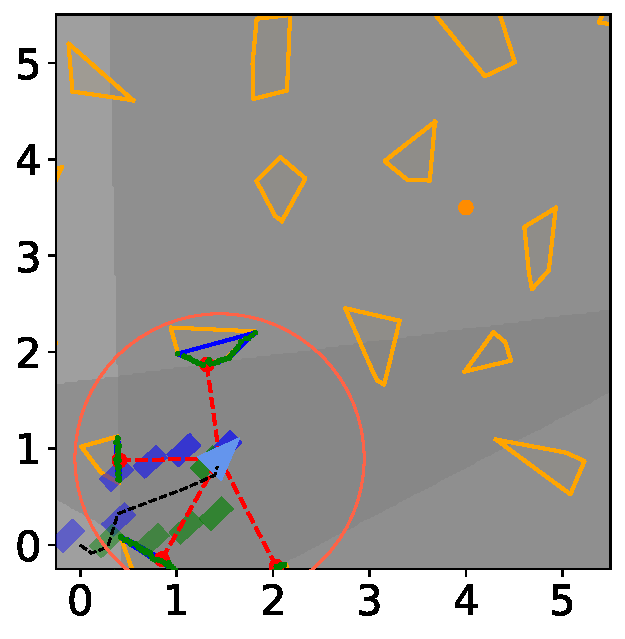
\includegraphics[width=\textwidth]{figures/Simulations/sim1/frame_3.pdf}
    \end{subfigure}%
    \hfill
    \begin{subfigure}{0.20\textwidth}
        \centering
        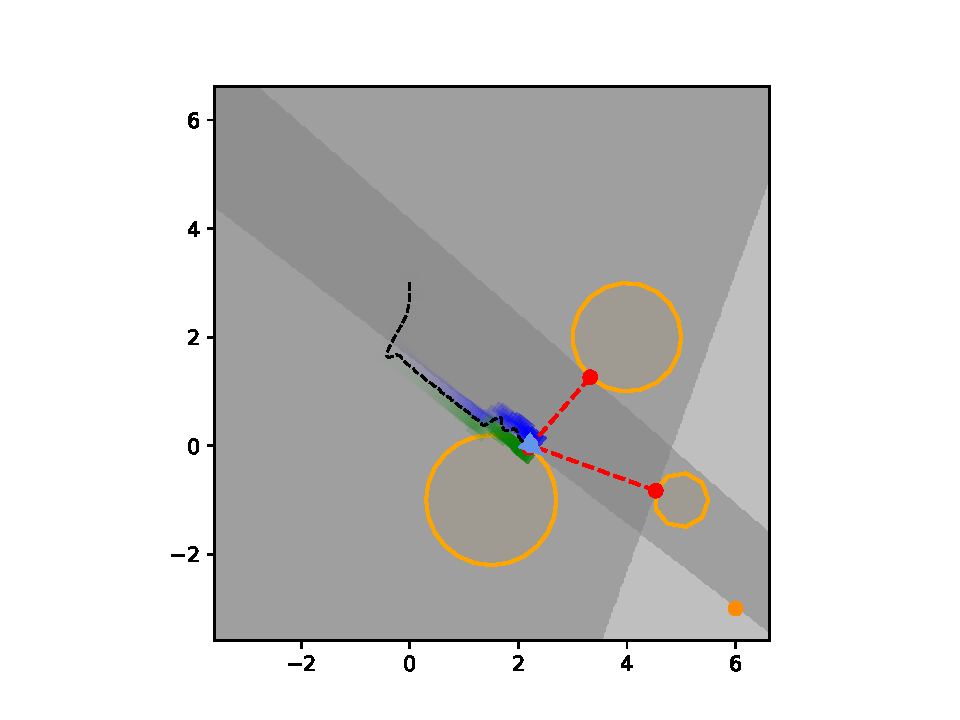
\includegraphics[width=\textwidth]{figures/Simulations/sim1/frame_4.pdf}
    \end{subfigure}
    
    % Second row
    \begin{subfigure}{0.20\textwidth}
        \centering
        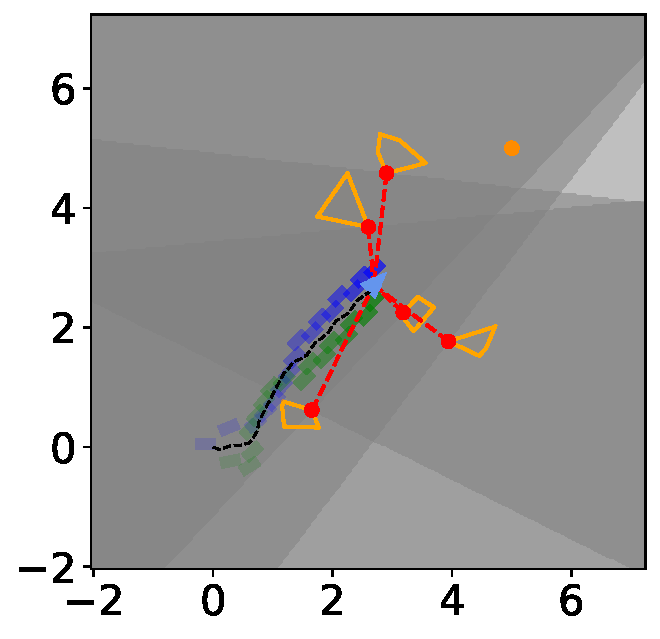
\includegraphics[width=\textwidth]{figures/Simulations/sim1/frame_5.pdf}
    \end{subfigure}%
    \hfill
    \begin{subfigure}{0.20\textwidth}
        \centering
        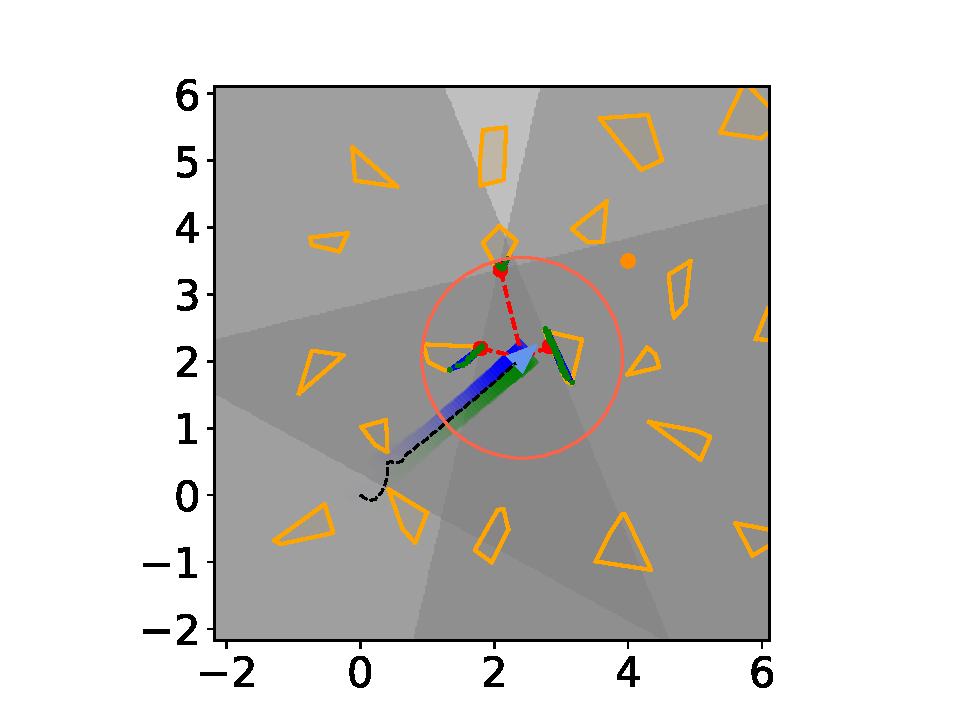
\includegraphics[width=\textwidth]{figures/Simulations/sim1/frame_6.pdf}
    \end{subfigure}%
    \hfill
    \begin{subfigure}{0.20\textwidth}
        \centering
        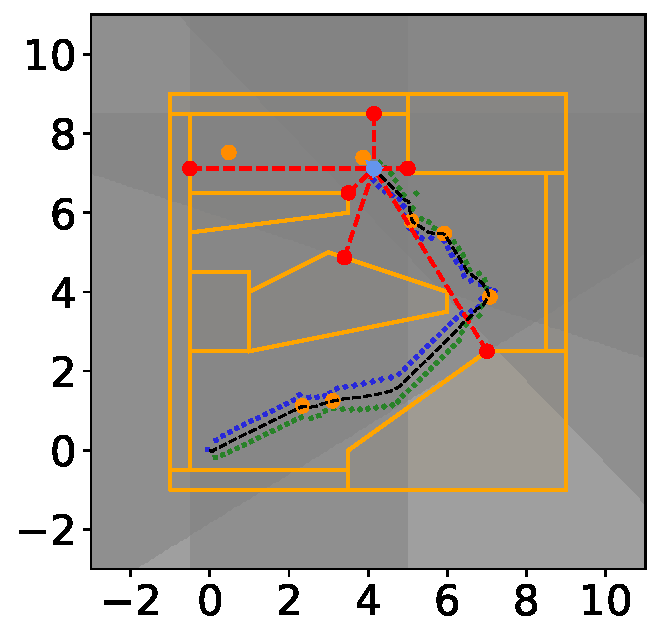
\includegraphics[width=\textwidth]{figures/Simulations/sim1/frame_7.pdf}
    \end{subfigure}%
    \hfill
    \begin{subfigure}{0.20\textwidth}
        \centering
        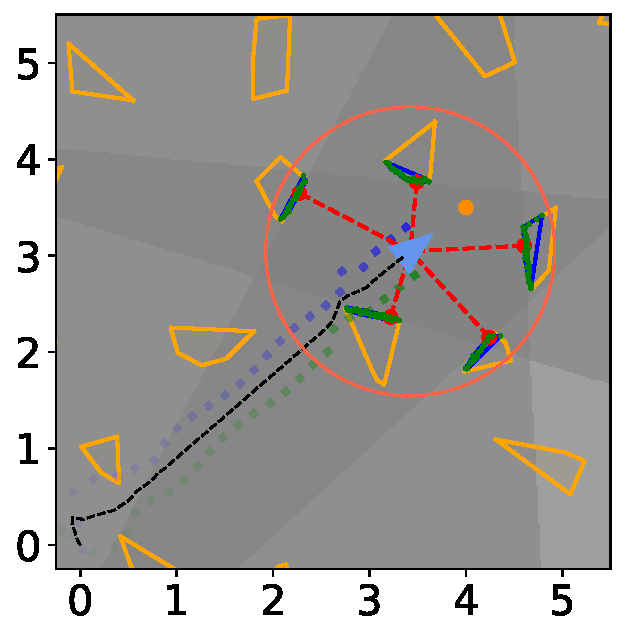
\includegraphics[width=\textwidth]{figures/Simulations/sim1/frame_8.pdf}
    \end{subfigure}%
    \hfill
    \begin{subfigure}{0.20\textwidth}
        \centering
        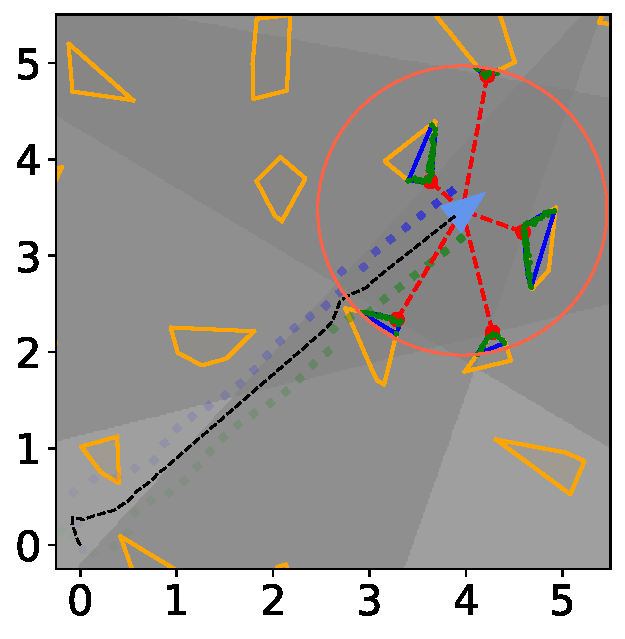
\includegraphics[width=\textwidth]{figures/Simulations/sim1/frame_9.pdf}
    \end{subfigure}
    
    \caption[short]{This is a description.}
\end{figure}

\end{document}